\subsection{Beveiligen van e-mail}

Het is mogelijk om beveiliging te voorzien op eender welke van de top vier lagen. Wanneer beveiliging wordt voorzien voor een specifieke applicatie -, transport -, netwerk laag protocol of op een koppeling basis, zullen de applicaties die gebruik maken van die protocol kunnen genieten van één of meerdere beveiligings diensten.
Waarom worden beveiligings functionaliteiten voorzien op meerdere lagen? Is het niet voldoende dat ze gedaan worden op de netwerk laag?
\begin{enumerate}
    \item	Hoewel beveiliging op de netwerk laag een “blanket coverage” kan aanbieden door alle data in de datagrammen te encrypteren en door alle bron IP adressen te authenticeren, kan het geen beveiliging voorzien op gebruikersniveau.
    \item Het is in het algemeen makkelijker om nieuwe internet diensten te implementeren,
    inclusief beveiligingsdiensten, op de hogere lagen van de protocol stack.
\end{enumerate}

\subsubsection{Alice wants to send confidential e-mail, m, to Bob.}

\begin{figure}[h]
    \centering
    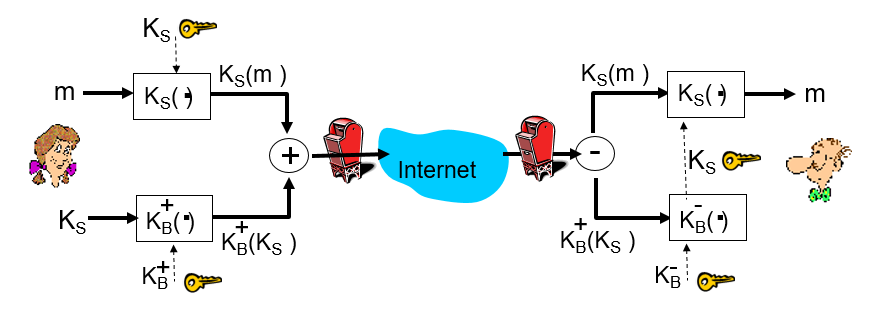
\includegraphics[width=4in]{./img/imghfdst8/hfdst8puntje23.png}
    \caption{Schema Alice wants to send confidential e-mail, m, to Bob }      
    \label{fig:Schema Alice wants to send confidential e-mail, m, to Bob }
\end{figure}

\noindent Alice:

\bi
\itf generates random symmetric private key, KS
\itf encrypts message with KS  (for efficiency)
\itf also encrypts KS with Bob’s public key
\itf sends both KS(m) and KB(KS) to Bob
\ei

\noindent Bob:

\bi
\itf uses his private key to decrypt and recover KS
\itf uses KS to decrypt KS(m) to recover m
\ei

\subsubsection{Alice wants to provide sender authentication and message integrity}

\begin{figure}[h]
    \centering
    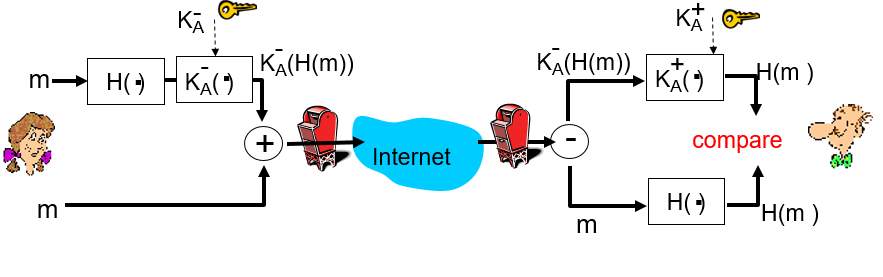
\includegraphics[width=4in]{./img/imghfdst8/hfdst8puntje24.png}
    \caption{Schema Alice wants to provide sender authentication and message integrity }      
    \label{fig:Schema Alice wants to provide sender authentication and message integrity }
\end{figure}

\bi
\itf Alice digitally signs message
\itf sends both message (in the clear) and digital signature
\ei

\subsubsection{Alice wants to provide secrecy, sender authentication,message integrity.}

\begin{figure}[h]
    \centering
    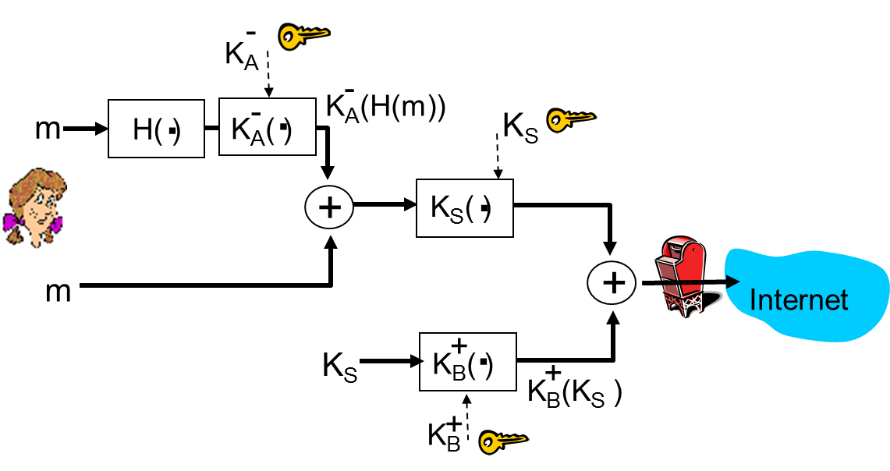
\includegraphics[width=4in]{./img/imghfdst8/hfdst8puntje25.png}
    \caption{Schema Alice wants to provide secrecy, sender authentication,message integrity }      
    \label{fig:Schema Alice wants to provide secrecy, sender authentication,message integrity }
\end{figure}

\noindent Alice uses three keys: 

\be
\itf her private key, 
\itf Bob’s public key,
\itf newly created symmetric key.
\ee
	



\subsubsection{Beveiligde e-mail}

Welke beveiligingskenmerken zouden het meest wenselijk zijn?

\begin{itemize}
\item \textbf{Confidentialiteit}: je wilt niet dat iemand anders het bericht leest.
\item \textbf{Zender authenticatie}: zeker zijn dat het bericht van de juiste zender komt.
\item \textbf{Bericht integriteit}: zekerheid dat het bericht niet is aangepast
\item \textbf{Ontvanger authenticatie}: dat het bericht ook bij de juiste ontvanger aankomt
\end{itemize}

\noindent De belangrijkste zorg is \textbf{confidentialiteit}. De meest eenvoudige manier om confidentialiteit te voorzien is om het bericht te encrypteren met een symmetrische sleutel. 

\noindent Maar hier komt een moeilijkheid bij van hoe de symmetrische sleutel de delen dat enkel de zender en ontvanger deze hebben. 

\noindent Een alternatieve benadering kan de publieke sleutel cryptografie zijn. Hier maakt de ontvanger zijn publieke sleutel beschikbaar, de zender gebruikt die sleutel om het bericht te encrypteren en zend het geëncrypteerde bericht naar de ontvanger. Dit is een goede oplossing als de zender zeker is dat publieke sleutel die van de ontvanger is. Er is enkel een probleem wanneer er een groot bericht geëncrypteerd moet worden.

\noindent We gaan dus gebruik maken van een sessie sleutel. 

\noindent De zender kiest een willekeurige symmetrische sessie sleutel, encrypt het bericht m met de sleutel, encrypt de sleutel met de publieke sleutel van de ontvanger, voegt het geëncrypteerde bericht en sleutel bij elkaar toe om een packet te vormen en zendt deze door naar de ontvanger. De ontvanger gebruikt eerst zijn privé sleutel om de sessie sleutel de decrypteren, en om vervolgens met de gedecryptte sessie sleutel het bericht te decrypteren.

\noindent De volgende stap is dat het systeem voorziet dat zowel zender authenticatie als bericht integriteit voorziet. Hiervoor kunnen we digitale handtekening en bericht-samenvatting gebruiken. De zender past een HASH functie H toe bij het bericht m om zo een bericht samenvatting te krijgen. De zender tekent het resultaat van de functie met zijn privé sleutel om zo de digitale handtekening te maken. Voegt vervolgens het originele bericht toe met de handtekening om een pakket te maken en om dit dan door te sturen naar de ontvanger. De ontvanger gebruikt de publieke sleutel van de zender op de getekende bericht-samenvatting en vergelijkt dit met het resultaat van zijn bewerking van zijn eigen HASH van het bericht.

\noindent Om een e-mail systeem te ontwerpen dat confidentialiteit, authenticatie en bericht integriteit voorziet kan gedaan worden om de twee bovenstaande stappen te combineren. De zender creëert eerst een voorlopig pakket dat bestaat uit het originele bericht samen met de digitaal gehandtekende hash van het bericht. Vervolgens wordt dit voorlopig pakket beschouwd als een bericht en encrypt deze met een zelfgekozen symmetrische sleutel.

\noindent Er is nog één belangrijk probleem dat nog moet worden aangepakt. Namelijk dat de zender en ontvanger de publieke sleutel van elkaar moeten opvragen. De verdeling van deze sleutels is een onbeduidend probleem. Zo kan men niet zeker zijn dat het de juiste publieke sleutel is. Dit kan opgelost worden door gebruik te maken van een CA.

\subsubsection{PGP (Pretty Good Privacy)}

\fra  Dit is een e-mailversleutelingsmethode dat nu een standaard geworden is.

\noindent \acrshort{pgp}-software gebruikt:

\bi
\itf MD5 of SHA voor het berekenen van de hash
\itf CAST, Triple-DES of IDEA voor het versleutelen van de symmetrische sleutel
\itf RSA voor de versleuteling van de openbare sleutel
\ei
	
\noindent Wanneer PGP is geïnstalleerd, maakt de software een openbare sleutel-combinatie voor de gebruiker. De openbare sleutel kan op de website van de gebruiker worden gepubliceerd of op een openbare sleutel-server worden geplaatst. De geheime sleutel is door een wachtwoord beschermd.

\noindent PGP geeft de gebruiker de keuze om het bericht:

\bi
\itf Digitaal te ondertekenen
\itf Te versleutelen
\itf Digitaal te ondertekenen en te versleutelen dus gecombineerd gebruiken.
\ei

\bi
\itf but want to send byte streams \& interactive data
\itf want set of secret keys for entire connection
\itf want certificate exchange as part of protocol: handshake phase
\ei

\begin{figure}[h]
    \centering
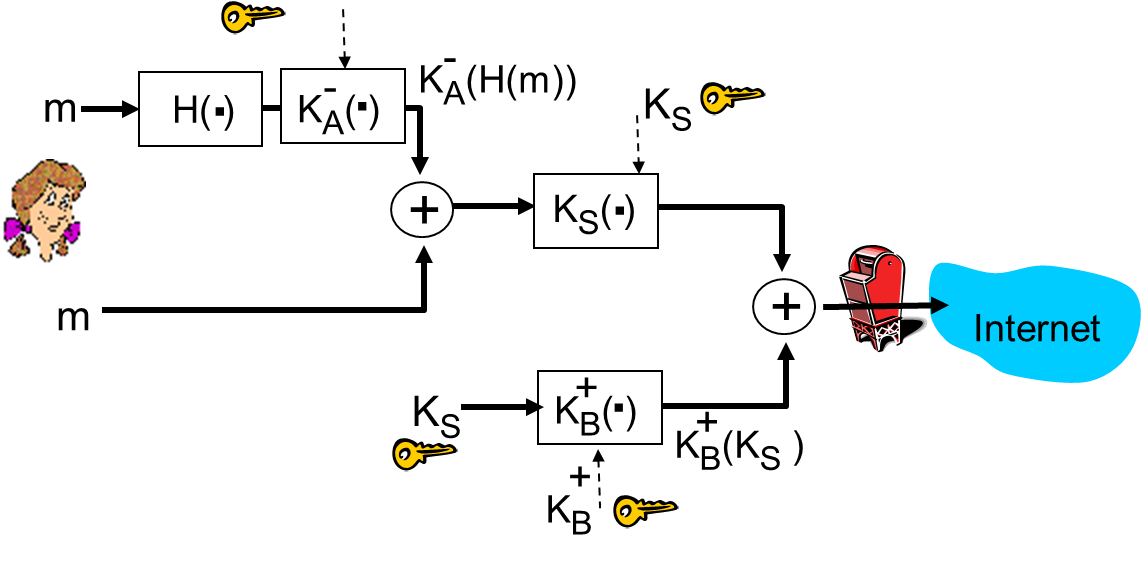
\includegraphics[width=4in]{./img/imghfdst8/hfdst8puntje26.png}
    \caption{PGP schema }      
    \label{fig:PGP schema }
\end{figure}

\noindent Is een e-mail encryptie schema dat een standaard is geworden. Afhankelijk van de versie, gebruikt de PGP software MD5 of SHA om de bericht-samenvatting te berekenen, CAST, 3-DES of IDEA voor de symmetrische sleutel encryptie en RSA voor de publieke sleutel encryptie.

\noindent Wanneer PGP geïnstalleerd is, creëert het een publieke sleutel paar voor de gebruiker. De publieke sleutel kan op de gebruikers website of in een publieke sleutel server geplaatst worden. De privé sleutel is beschermd door het gebruik van een wachtwoord die elke keer moet ingegeven worden als die sleutel gebruikt wil worden.

\noindent PGP geeft de mogelijkheid om een bericht digitaal te handtekenen, het bericht te encrypteren of zowel handtekenen als encrypteren.

\noindent PGP voorziet ook een mechanisme voor publieke sleutel certificatie, maar dit mechanisme is wat anders dan de meer conventionele CA. PGP publieke sleutels zijn gecertificeerd door een web of trust. 

\noindent Een persoon kan zelf elk sleutel/gebruikersnaam paar certificeren wanneer ze gelooft dat het paar echt bij elkaar hoort. In toevoeging laat PGP toe dat als een persoon een ander persoon vertrouwt om in te staan voor de authenticatie van meer sleutels.